%!TEX program = xelatex

%# -*- coding: utf-8-unix -*-
%%==================================================
%% thesis.tex
%%==================================================

% 双面打印
\documentclass[master, fontset=adobe, openany, twoside]{sjtuthesis}
% \documentclass[bachelor, fontset=adobe, openany, oneside, submit]{sjtuthesis} 
% \documentclass[master, adobefonts, review]{sjtuthesis} 
% \documentclass[%
%   bachelor|master|doctor,	% 必选项
%   fontset=adobe|windows,  	% 只测试了adobe
%   oneside|twoside,		% 单面打印,双面打印(奇偶页交换页边距,默认)
%   openany|openright, 		% 可以在奇数或者偶数页开新章|只在奇数页开新章(默认)
%   zihao=-4|5,, 		% 正文字号:小四、五号(默认)
%   review,	 		% 盲审论文,隐去作者姓名、学号、导师姓名、致谢、发表论文和参与的项目
%   submit			% 定稿提交的论文,插入签名扫描版的原创性声明、授权声明 
% ]

% 逐个导入参考文献数据库
\addbibresource{bib/thesis.bib}
% \addbibresource{bib/chap2.bib}

\begin{document}

%% 无编号内容:中英文论文封面、授权页
%# -*- coding: utf-8-unix -*-
\title{Sandboxing 相关技术研究与思考}
\author{尹至达}
\advisor{高\quad{}策}
\defenddate{2016年12月30日}
\school{上海交通大学}
\institute{某某系}
\studentnumber{116037910012}
\major{116037910024}

\maketitle

\frontmatter 	% 使用罗马数字对前言编号

%% 摘要
\pagestyle{main}
%# -*- coding: utf-8-unix -*-
%%==================================================
%% abstract.tex for SJTU Master Thesis
%%==================================================

\begin{abstract}

目前,互联网上的攻击越来越频繁,攻击者会通过各种攻击方式,以达到获取系统高权限,读取敏感数据等等攻击目的。沙箱作为一个用来隔离程序执行环境,使得程序在一个低权限的,高度隔离的环境中执行的技术,受到了越来越多的关注。本文以一个现代的浏览器为出发点,介绍了两类沙箱技术在其中的应用与体现,进而总结对比各种沙箱实现的特点,并且在最后对沙箱技术下一步的研究方向提出了看法。

\keywords{\large Sandboxing \quad Capabilities \quad Software-based Fault Isolation \quad System Call Interposition}
\end{abstract}


%% 目录、插图目录、表格目录
\tableofcontents

\mainmatter	% 使用阿拉伯数字对正文编号

%% 正文内容
\pagestyle{main}
%# -*- coding: utf-8-unix -*-
%%==================================================
%% chapter01.tex for SJTU Master Thesis
%%==================================================

%\bibliographystyle{sjtu2}%[此处用于每章都生产参考文献]
\chapter{引言}
\label{chap:intro}

随着网络全球化的发展,网络安全进入了大众视野,成为一个越来越引人注目的议题。互联网在提供给用户以便利的同时,也对隐私安全提出了新的挑战。这样的问题存在于各种平台上,攻击者会将诸如木马、病毒、恶意软件等等内容发布到被攻击者的终端上 \parencite{miwa}。虽然现在的操作系统上的安全措施已经足够强大到防止绝大多数的攻击,但是用户总是期望更加安全的环境。而沙箱是一种非常实用的安全机制,通过引入沙箱技术,程序可以在隔离的环境中运行,使得程序的运行不会影响操作系统,同时操作系统也不会影响到程序。在传统的操作系统的抽象中,用户的应用对于系统各种资源的使用都是无限制的,而沙箱技术是对其运行时环境的隔离 \parencite{sandbox}。

% \begin{figure}
% \centering
% \subfloat[第一类沙箱]{
% \label{fig:t1sb}
% 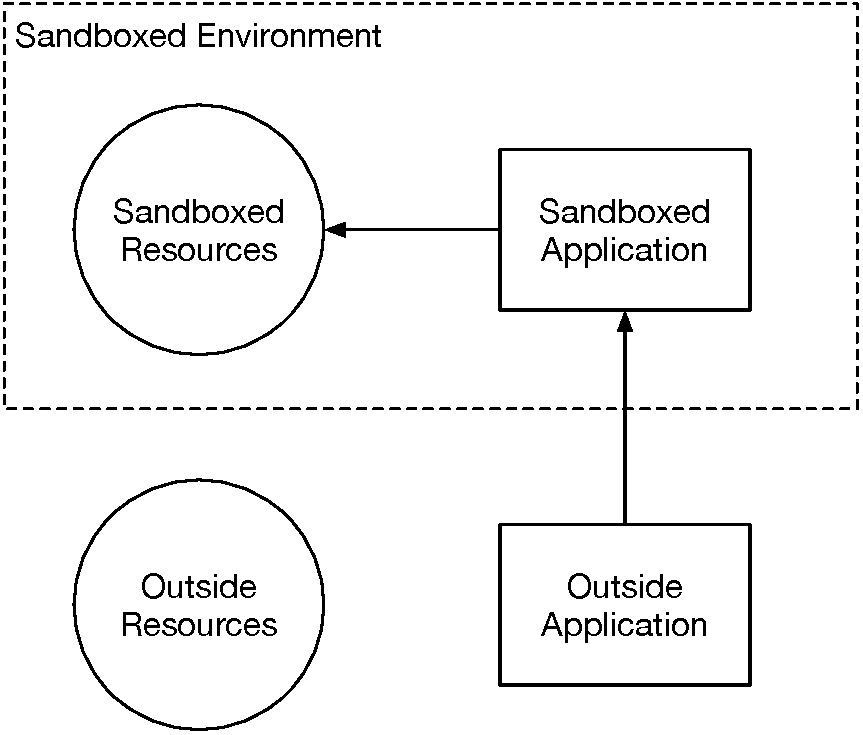
\includegraphics[width=0.3\linewidth]{imgs/type-1-sandbox}
% }
% \subfloat[第二类沙箱]{
% \label{fig:t2sb}
% 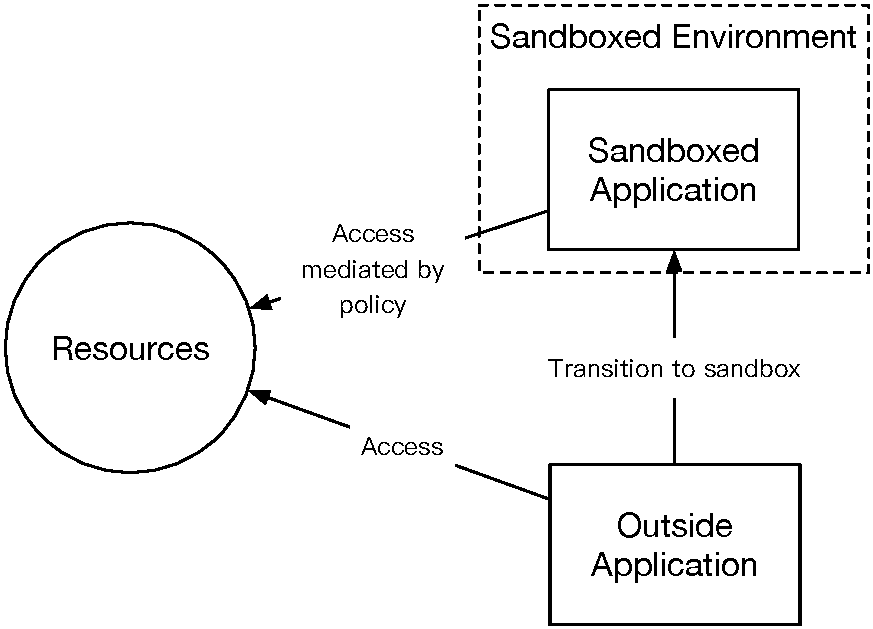
\includegraphics[width=0.3\linewidth]{imgs/type-2-sandbox}
% }
% \caption{沙箱分类}
% \end{figure*}

\begin{figure}[!htp]
  \centering
  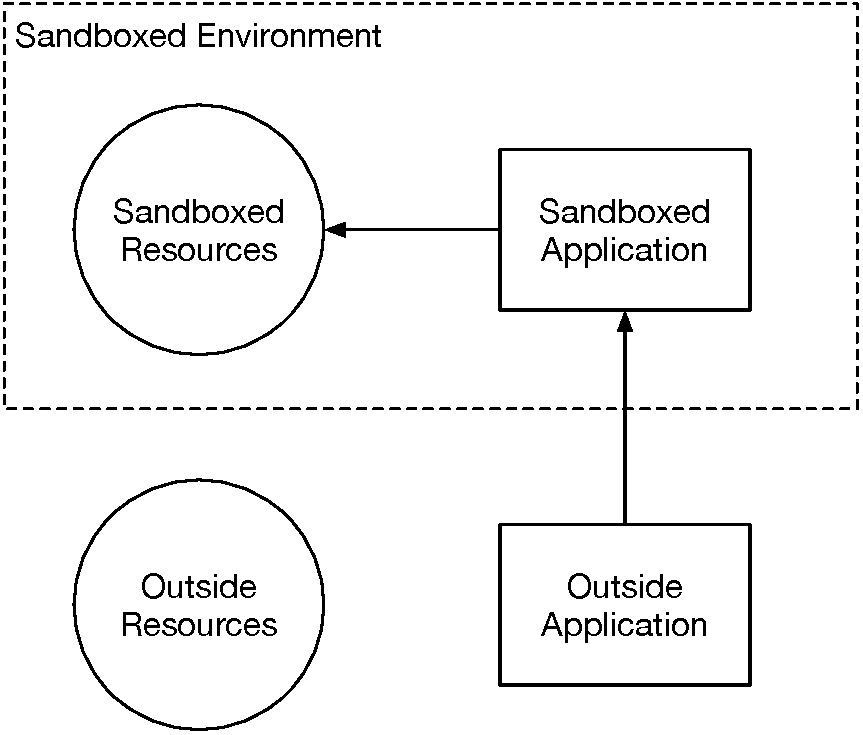
\includegraphics[width=0.35\textwidth]{imgs/type-1-sandbox}
  \caption{第一类沙箱}
  \label{fig:t1sb}
\end{figure}

\begin{figure}[!htp]
  \centering
  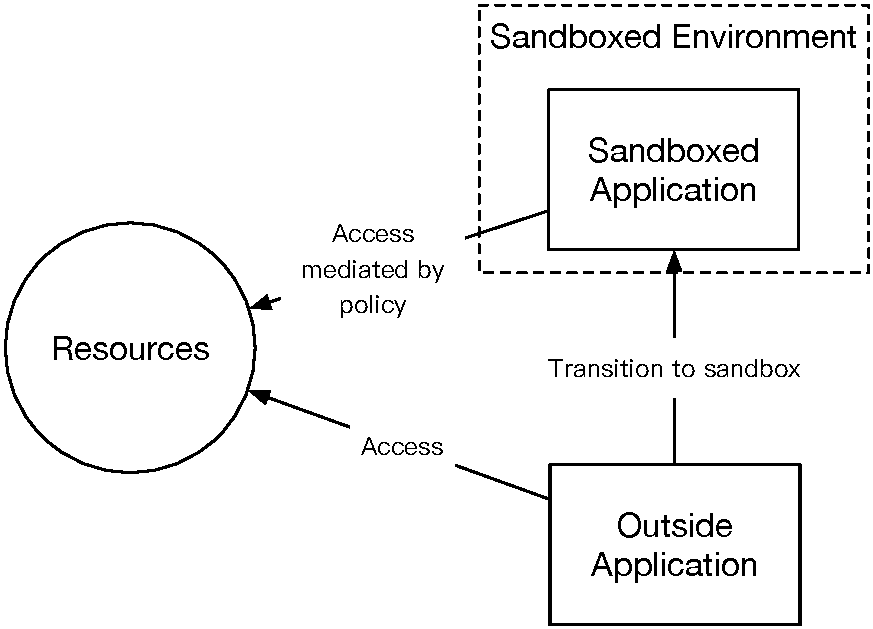
\includegraphics[width=0.35\textwidth]{imgs/type-2-sandbox}
  \caption{第二类沙箱}
  \label{fig:t2sb}
\end{figure}

沙箱技术大致可以被分为两类,其中第一类是基于隔离的沙箱,该类型的沙箱将应用的执行环境从操作系统中隔离出来,形成一个独立的执行环境。图 \ref{fig:t1sb} 展示了一个经典的基于隔离的沙箱模型。一个应用程序会在启动另一个应用程序之前先启动应用程序的沙箱,然后在沙箱内运行该应用程序,沙箱内的应用程序只能访问到沙箱内的资源。广为人知的虚拟机,容器,和传统意义上的沙箱都是这一类的沙箱模型。

第二类是基于规则的沙箱,该类型的沙箱并不是完全关注于对于应用程序的隔离上,而是用规则的方式控制每个应用的权限,基于规则的沙箱之间可以分享操作系统的逻辑资源。图 \ref{fig:t2sb} 展示了第二类的沙箱模型,不同于基于隔离的沙箱模型的地方在于,基于规则的沙箱模型并没有实现完全的资源隔离,而是对于每个应用,有不同的限制策略,通过强制应用限制策略来保证资源的访问权限受控 \parencite{schreuders}。

由于篇幅限制,本文不能面面俱到地对各种沙箱技术都予以介绍,为了保证深度,本文选取第一类沙箱中的 Software-based Fault Isolation,以及第二类沙箱中的 System Call Interposition 和 Capabilities,来介绍沙箱技术的应用场景与实现,以及各自的优缺点,并在文末展开对各种技术的实现原理和潜在研究点的讨论。

%# -*- coding: utf-8-unix -*-
%%==================================================
%% chapter02.tex for SJTU Master Thesis
%% based on CASthesis
%% modified by wei.jianwen@gmail.com
%% Encoding: UTF-8
%%==================================================

\chapter{威胁模型}
\label{s:threat_model}

目前在互联网上,不受信任的应用的数量正在快速增长,让不受信任的应用程序能够更好地运行在系统中,是一件相当困难的事情。这些不受信用的应用程序可能隐藏有带有攻击意图的代码,它们获取操作系统高权限、读取文件系统中的敏感数据(比如密码、照片、文档等)、植入广告、导致系统崩溃等等。而攻击手段有很多,其中包括代码注入、Cross Site Scripting(CSS)、缓冲区溢出、Return-oriented programming(ROP) 等等 \parencite{miwa}。	

传统的操作系统并没有很好地解决这方面的问题,在隔离方面,仅仅依靠运行时的简单隔离是不够的。新的趋势使得操作系统应该在处理器,内存等硬件层面和进程,文件系统等软件层面进行更加细致的隔离和容错。这也是沙箱技术关注的焦点。不同的沙箱技术针对的威胁模型都是不一样的,但是它们在宏观上都有一个共同点:防止不受信任的应用程序可以随意访问地操作系统或者底层的硬件。

\chapter{Sandboxing 相关技术以及使用场景}
\label{s:implementation}

为了能够深入浅出地进行介绍,方便理解,本节将以一个现代的浏览器作为应用场景进行切入,在浏览器上,沙箱有着非常多的应用:

\begin{itemize}
\item
网页应用,现代的浏览器会在沙箱中运行你打开的网页代码。诸如 Javascript 之类的网页代码在浏览器的沙箱中只有有限的权限,它们并不能直接与文件系统等等进行交互,因此 Javascript 中的恶意代码的破坏性仅限于在沙箱内。
\item
浏览器插件,浏览器并不会直接将插件进程运行在操作系统上,而是会将其运行在一个沙箱进程中。比如 Adobe Flash 插件,就是如此。这样的隔离方式使得插件如同网页应用一样不能直接与操作系统进行交互,防止两者之间相互的攻击。
\item
各类下载内容的查看器,以 PDF 文件为例,浏览器下载的 PDF 文件会使用系统内的 PDF 阅读器打开,目前一些 PDF 阅读器正在使用沙箱技术来解析 PDF 文件,其中最有名的是 Adobe Reader。它运行在一个沙箱中,因此如果 PDF 文件中有恶意内容,也不会影响到操作系统。
\item
浏览器本身,浏览器是沙箱技术运用最广泛的桌面应用之一。浏览器不止将其请求的网页应用和插件等运行在容器中,浏览器本身也是运行在一个独立而隔离的沙箱中的。低权限的沙箱运行可以保证即使恶意内容破坏了网页应用所在的沙箱,也会被浏览器的沙箱所限制 \footnote{http://www.howtogeek.com/169139/sandboxes-explained-how-theyre-already-protecting-you-and-how-to-sandbox-any-program/}。
\end{itemize}

本节将介绍 System Call Interposition(SCI)、Software-based Fault Isolation(SFI) 和 Capabilities 等技术在浏览器中的体现。System Call Interposition(SCI) 通过对系统调用的跟踪和限制,来使得应用不可以调用一些敏感的系统调用,或者不能将敏感的参数传入到系统调用中。Software-based Fault Isolation(SFI) 更加关注如何在一个应用程序产生了故障后,不会影响到其他的应用程序,同时保证应用程序之间的数据和代码是不能被彼此访问到的。Capability Security Model(CSM)是一种区别于对服务提供者进行诸如Acccess Control List(ACL)的权限检查,而将权限检查绑定在被需要的实体上的一种设计理念 \footnote{http://wiki.c2.com/?CapabilitySecurityModel}。这是三种完全不同的思路,它们的目的都是隔离代码的运行环境,构建出一个高度隔离的,低特权级的沙箱环境。

\section{System Call Interposition(SCI)}
\label{ss:sci}

在浏览器中,有很多互联网上的内容是需要下载,然后使用本地的查看器打开的。比如 PDF 文件等,需要通过 Adobe Reader 等专用软件打开。但是下载的内容有可能是隐藏有恶意代码的,但是本地的查看器并不一定将其视为不可信的内容,因此下载的内容在被相应的查看器打开时,恶意代码可能会被错误地执行了。对 System Call Interposition(以下称为 SCI)的研究,起初的动机是如何限制打开浏览器下载内容的助手应用,希望能够限制助手应用本身进行系统调用的权限。它的思想是通过监控和审查应用程序进行的系统调用,保证其不能顺利进行系统不允许其进行的系统调用。SCI 的思想参考了 Unix 的最小特权原则,所有应用程序都应该被授予其需要的权限组成的最小集合。本节将以 Janus 和 Ostia 作为主要内容,介绍 SCI 的思想和实现。

\subsection{Janus}
\label{sss:janus}

Janus \parencite{goldberg} 是 Goldberg 在 1996 年发表的论文,也是第一个成型的 SCI 系统实现,是这一领域奠基性的论文。Janus 最初的动机是限制助手应用的权限,其提出了几种可能的实现方法。其中包括:

\begin{itemize}
\item
在每个助手应用中单独地实现自己的安全保护。这是第一个被排除的选择,这样的实现会使得应用的实现变得更加复杂,而且应用的提供商未必有动力去实现完全的安全保护。而很多应用是闭源的,因此成本极大。从另一方面来讲,安全可以在更加底层的角度来实现。
\item
在操作系统中加入新的安全特性。所有的应用程序都是运行在操作系统之上的,因此只要在操作系统层面实现了安全策略,那所有的应用程序都会受益。但是 Janus 最后没有采取这样的方法,因为开发和维护这样的特性是需要修改内核的,很多用户不希望自己在添加安全保护的时候需要请系统管理员来为自己的操作系统打补丁。而且在内核中的修改是特别危险的,内核中的 bug 往往会造成更加严重的安全事故。
\item
使用已有的 reference monitor。传统操作系统中的 monolithic 的 reference monitor 不能保护应用程序不会被攻击,而只能保证攻击不会很快的传播。
\item
传统的网络防火墙。这样的思路实现起来会非常复杂,因为这样的一个过滤器或者代理需要支持所有的文件格式等等。
\end{itemize}

因此,在分析了现有的思路都不能满足需求后,Janus 的作者提出了一种新的思路,一种在用户态实现安全的方法。它的实现不要求修改操作系统和应用程序,而只是在用户态实现了一个 policy engine,进而对于每一个应用程序指定一个安全策略,由 policy engine 来保证安全策略会被应用在应用程序运行时。

\begin{figure}[!htp]
  \centering
  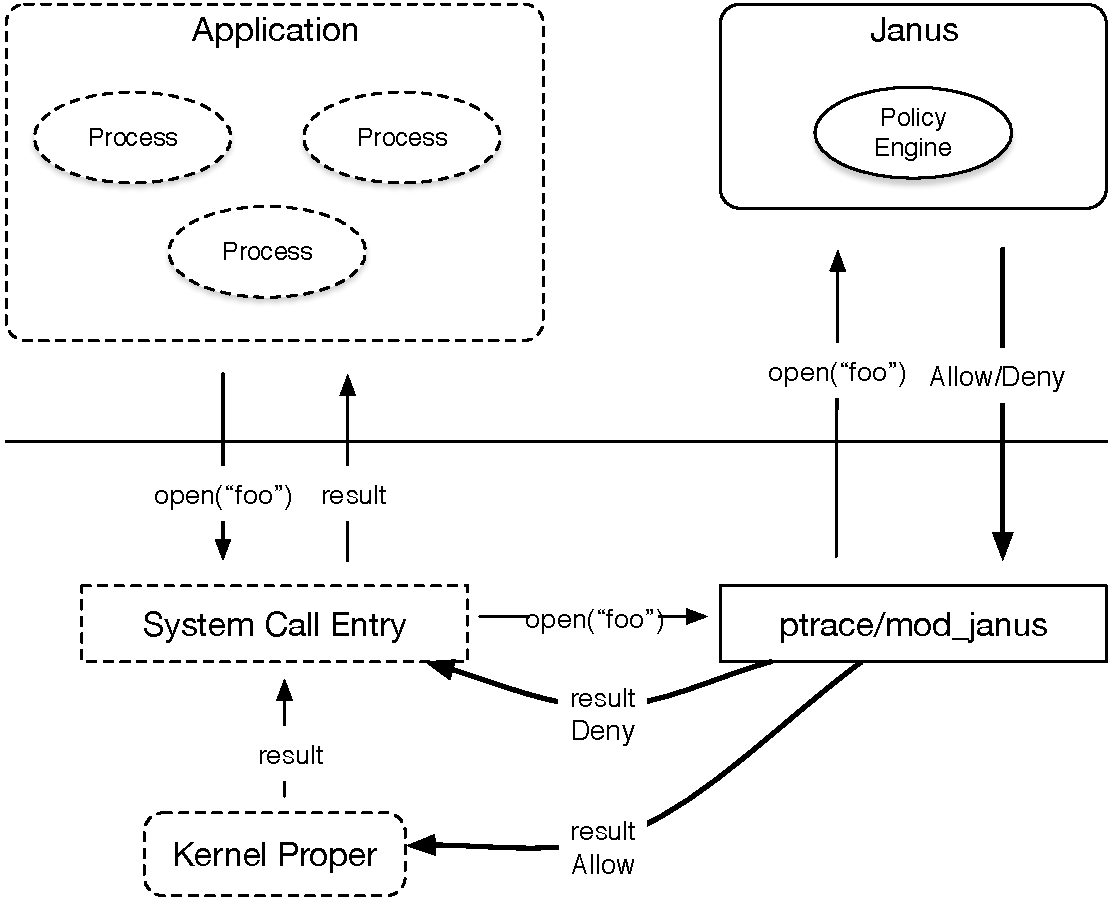
\includegraphics[width=0.7\linewidth]{imgs/janus}
  \caption{Janus 架构图}
  \label{fig:janus}
\end{figure}

在设计架构时,Janus 主要考虑了三点:

\begin{itemize}
\item
安全,这也是最基本的原则。Janus 保证应用程序不能访问它没有权限访问的系统或者网络。为了更加地安全可靠,Janus 认同 "keep it simple" 的理念 \parencite{keepitsimple}。Janus 认为只有简单的实现才能使得其更加安全。
\item
灵活,Janus 不仅可以做到在系统调用的粒度实现拦截与过滤,同时希望在更加细致的粒度,比如系统调用的参数等粒度上同样可以进行请求的拦截与过滤。
\item
可配置,Janus 应该用户针对不同的应用程序进行不同的策略定制。
\end{itemize}

为了实现上述三点,Janus 进行了如图 \ref{fig:janus} 所示的架构设计。其中由 Janus 负责实现的只有右上角的 policy engine,其他是由操作系统或者应用程序来实现的。当一个应用程序被启动时,Janus 会读取该应用程序的配置文件,随后会 fork 一个子进程,在子进程中运行应用程序,并且会调用 ptrace 来监控应用程序子进程的系统调用。子进程会 exec 应用程序,每当有系统调用时,会交由 policy engine 来决定应用程序是否有权利进行此次系统调用。

通过借助内核中已有的特性:ptrace,Janus 非常简单地实现了 policy engine,相比于传统的应用程序执行流程,Janus 在操作系统之上,在用户态创建了一层新的抽象,这层抽象会负责进行系统调用的拦截和过滤,保证应用程序的隔离。

但是,后续的研究发现这样的实现是不完整的。Wagner 在1999年的论文中提到 \parencite{wagner1999janus},ptrace 会导致 Janus 的一些缺点。最大的问题在于,当 Janus 进行安全检查拒绝了此次系统调用的请求时,ptrace 不支持拒绝此次请求,而只能以杀掉子进程的方式进行。在日常的使用中,几乎所有的应用都会有一些在配置文件中不允许其进行的系统调用,而杀掉进程的方式对于应用程序来说并不是合适的做法。因此 Janus 在后续的版本中实现了一个内核的模块,该模块替换了 ptrace,解决了这一问题。

除此之外,Janus 还有很多其他的问题,比如:

\begin{itemize}
\item
会错误地对操作系统的状态进行保存。为了确定是否响应请求,Janus 在 policy engine 中会保存一些操作系统的运行状态,而这会导致不一致的发生。
\item
忽略间接的对文件系统的访问。虽然 Janus 会监控应用程序对文件系统的访问,但是有一些间接的访问是很难防止。举例说明,当应用程序以 core dump 的方式创建一些文件时,Janus 并没有办法禁止其对文件系统的操作。
\item
数据竞争。因为在用户态的 policy engine 和在内核态的系统调用不是原子性的,数据竞争就有可能发生。这是比之前两个都要严重的问题,也是 SCI 的另一实现,Ostia 试图解决的问题\parencite{garfinkel2003traps},这将在下一节中详细介绍。
\end{itemize}

\subsection{Ostia}
\label{sss:ostia}

在 Janus 之后,有很多相关研究就此展开,研究者们继续完善 Janus,并且提出了新的解决思路。Ostia \parencite{garfinkel} 是 2004 年被提出的,它指出 Janus 存在很多缺点,而这些缺点的产生是因为架构问题,而不是 SCI 所固有的。因此它提出了一种新的架构,并且验证了他们的工作是比 Janus 的实现要高效而且可以解决 Janus 的缺点与问题。

Ostia 认为,以  Janus 为代表的 SCI 实现最大的问题在于,Janus 可能会导致数据竞争。但是,这个问题并不是 SCI 这样的思想带来的,而是与 Janus 的实现有关的。所以 Ostia 提出了基于委托的架构,Janus 是基于过滤的架构,而 Ostia 的架构与其不同,如图 \ref{fig:ostia} 所示,Osita 在应用程序的进程中多了一个组件,即 emulation library。对于每一个应用程序,都有一个 agent 与之对应。在 Janus 中,因为应用程序是被监控的程序,所以需要由 Janus 创建一个新进程,再执行应用程序的逻辑。与之类似的是,Ostia 实现了一个 ELF 格式的二进制加载器,在加载应用程序时,它同时还会加载 emulation library 到应用程序的内存空间中。整个的实现是回调的机制,当有一个敏感的系统调用被执行时,内核会把请求重定向到跟调用的进程在同一内存空间的 emulation library 中的 handler 处理,handler 会将请求转发给 agent,随后再有 agent 进行权限的校验,在校验成功后会发送真正的请求。

\begin{figure}[!htp]
  \centering
  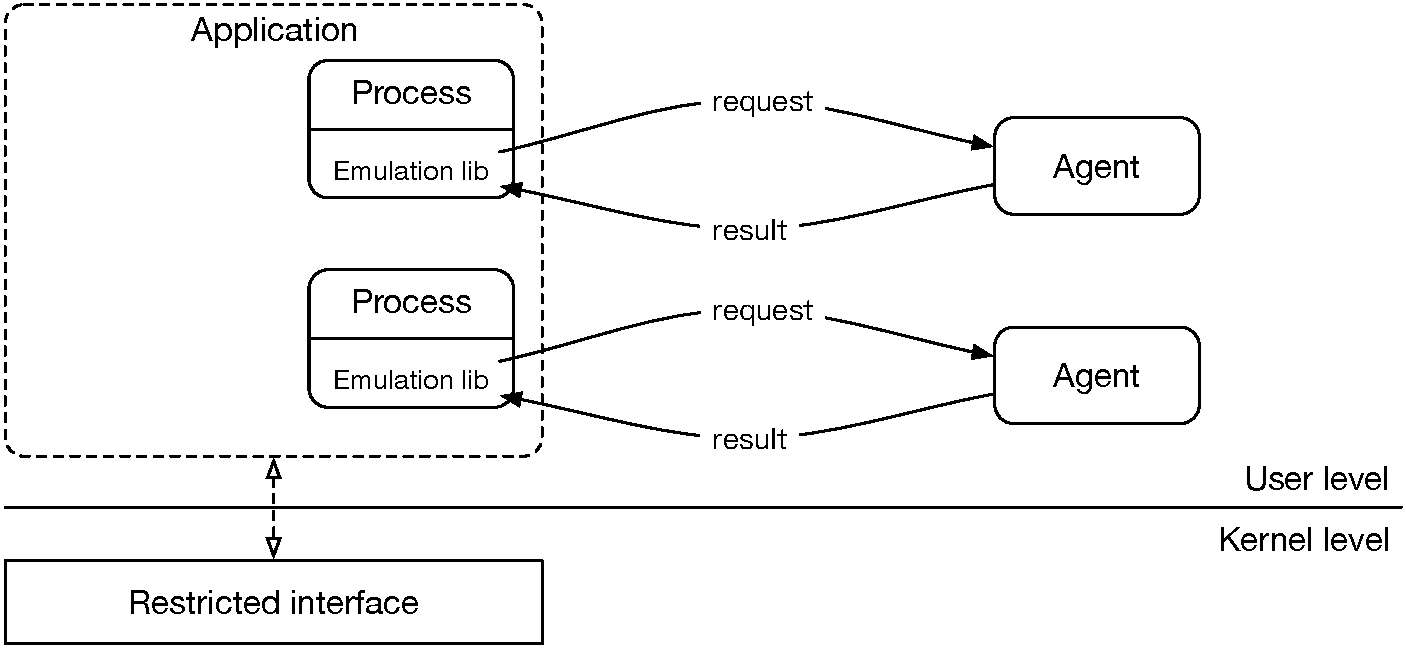
\includegraphics[width=0.8\linewidth]{imgs/ostia}
  \caption{Ostia 架构图}
  \label{fig:ostia}
\end{figure}

因此,所有敏感的系统调用,都会被重定向到 agent 中进行处理,这样的架构在 Ostia 中被称为委托代理架构。Ostia 可以解决一部分 Janus 不能解决的数据竞争问题。

\section{Software-based Fault Isolation(SFI)}
\label{ss:sfi}

浏览器是一个泛用性很强的应用,因此浏览器要求支持以插件的方式进行功能扩展。同时,为了提高浏览器中代码执行的性能,目前很多浏览器都在探索在浏览器中执行 Native 代码的方法。其中谷歌浏览器支持将 Native 代码运行在一个使用 Software-based Fault Isolation(以下称为 SFI) 的沙箱中。SFI 是在 1994 年在 Wahbe 的论文中第一次出现的 \parencite{wahbe1994efficient},SFI 通过修改程序二进制的方式,使得程序的二进制代码符合一些规则,来完成对于错误的隔离。在后来的论文中,谷歌结合了 SFI 和其他的一些沙箱技术,实现了一个面向 Native 代码运行环境的沙箱,这项技术一直到现在仍在被谷歌 Chrome 浏览器使用 \parencite{nacl}。

\subsection{Efficient Software-based Fault Isolation}
\label{sss:esfi}

Fault Isolation 是一个在计算机科学领域存在已久的定义。在这篇论文发表之前,操作系统已经在软件和硬件层面都进行了 Fault Isolation 的实现。Remote Procedure Call(以下称为 RPC)实现了两个不同的进程间互不影响的通信,而使用不同的虚拟内存空间使得错误不会在两个进程中传播。但是这样的实现中,两个进程进行通信的成本是非常高的。

\begin{figure}[!htp]
 \centering
 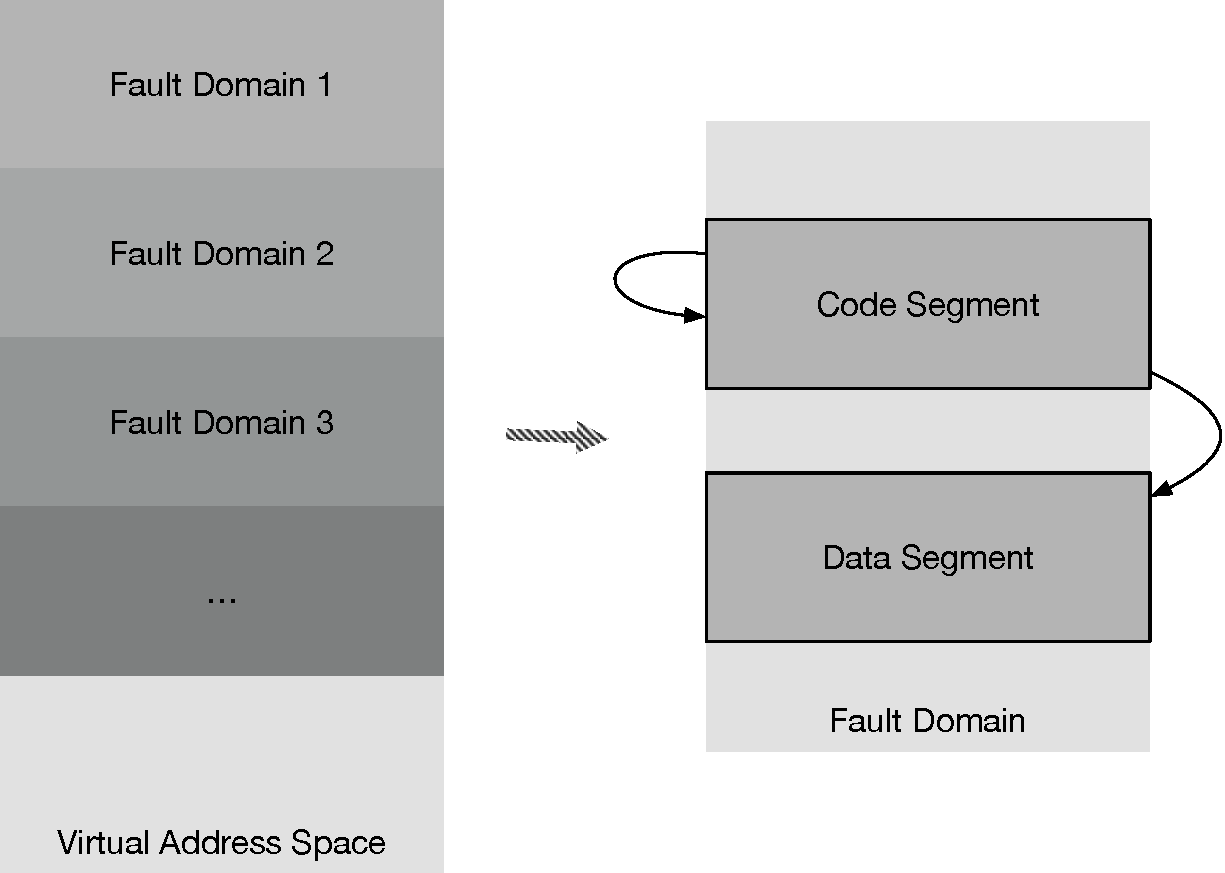
\includegraphics[width=0.8\linewidth]{imgs/sfi}
 \caption{Software-based Fault Isolation}
 \label{fig:sfi}
\end{figure}

这一篇论文第一次使用沙箱一词来描述基于软件的错误隔离机制,希望能够在同一地址空间中实现错误的隔离,这样就可以大大减小通信的开销。同一虚拟内存空间被划分成若干个 Fault Domain,每个 Fault Domain 都有自己的数据段和代码段,图 \ref{fig:sfi} 阐述了这篇论文的实现思路,对于每个 Fault Domain 而言,其只能在自己的代码段中进行控制流的转移,与此同时也只能访问自己的数据段 \parencite{wahbe1994efficient}。

SFI 的实现,使用了处理器的段寄存器。段寄存器最初是为了解决 Intel 8086 处理器体系架构中数据总线与地址总线的宽度不一致而引入的,因为不一致导致寻址不能在单个指令周期内完成,因此 Intel 引入了段寄存器,将整个内存空间分为了4个段,段寄存器存放每个段的前 N 位的地址,使用段内偏移量,而不是全部的物理地址来描述内存地址,解决了这一问题\footnote{https://en.wikipedia.org/wiki/X86\_memory\_segmentation}。在目前处理器的架构中,不再存在地址宽度不统一的问题,因此内存分段成为了可选的特性。而 SFI 通过对段寄存器的访问限制,将程序的控制流严格地限制在一个 Fault Domain 的代码段中。在进行控制的跳转时,会强制使用段寄存器进行检测,如果访问的地址的前 N 位与段基地址不一致,则会触发异常,说明应用程序正在尝试逃出自己的 Fault Domain。

SFI 的隔离实现,相比于传统的方式有着更小的 overhead,同时也开创了一种新的隔离机制。

\subsection{Native Client}
\label{sss:nacl}

Native Client 是谷歌 Chrome 浏览器上的一个特性,开发者可以通过它在浏览器中运行原生的程序,以解决以 Javascript 为代表的浏览器端代码执行效率慢的问题。严格来说 Native Client 结合了 SCI, SFI 等多种技术,进行了实现。

插件程序是各种主流浏览器都有支持的扩展方式,通过插件的方式,用户可以为自己的浏览器增添新的特性与功能。微软的 ActiveX 是最著名的插件支持,在用户浏览网页时,IE 浏览器可以自动下载网页上的 ActiveX 控件,增强网页的功能。但是 ActiveX 也因为漏洞多而饱受争议,所有的控件拥有访问 Windows API 的权力,这使得操作系统的安全受到了很大的挑战。而 Native Client 希望将插件运行在一个隔离可控的沙箱中,用沙箱来限制插件的执行环境。

\begin{figure}[!htp]
  \centering
  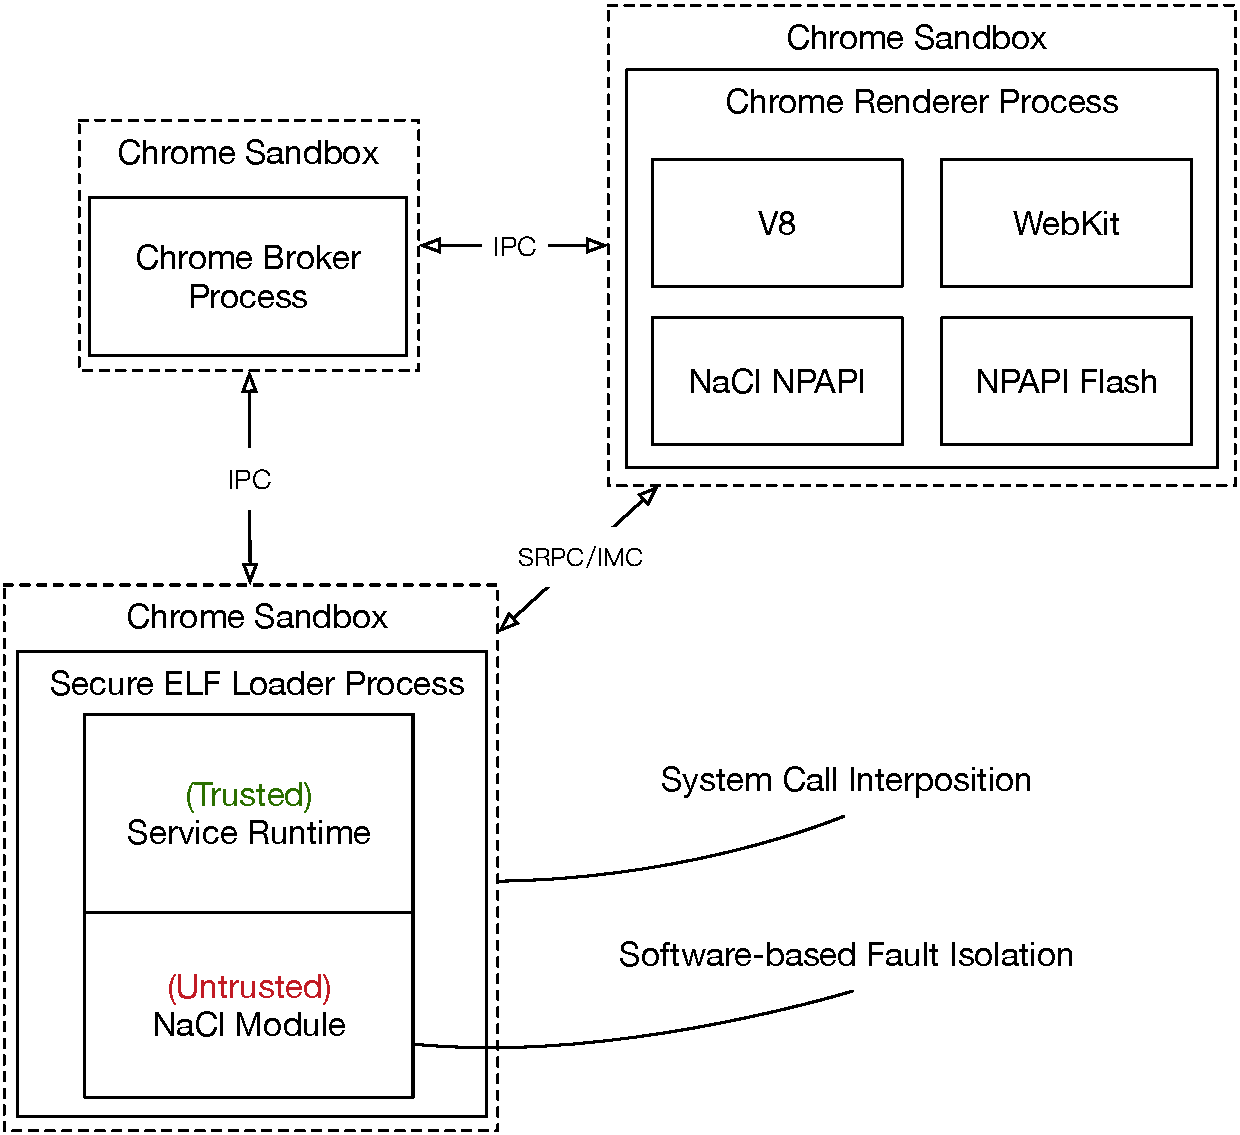
\includegraphics[width=0.65\linewidth]{imgs/nacl}
  \caption{Native Client 架构图}
  \label{fig:nacl}
\end{figure}

Native Client 使用了两层沙箱的架构,内层沙箱使用了 SFI 的技术,外层沙箱使用了 SCI 的技术。Native Client 相比于之前的实现,最大的贡献是改进了 SFI 的实现,减小了其在运行时的 overhead。图 \ref{fig:nacl} 中的 Native Client Module,即原生的插件代码。这一部分是通过谷歌修改过的 LLVM 或者 gcc 工具链编译出的二进制程序,在编译时会保证一定的规则,比如在跳转时进行段寄存器的校验等等 SFI 相关的指令检查。这是内层沙箱,这一层沙箱保证了原生的插件代码只能在自己的 Fault Domain 中运行。外层沙箱是由 Systrace \parencite{provos2003improving} 提供的类似上文中提到的 Janus 和 Ostia 的系统调用拦截的特性。

在之前的 SFI 实现中,为了在跳转时检查控制流的转移是否合法,需要额外的14个字节的指令。而在 Native Client 中,通过使用对齐的内存,使得跳转指令只能跳转到在32字节对齐的地址段中的第一个地址处。因此,在跳转时的检查由原本的14个字节的指令变成了8个字节的指令。这也是 Native Client 对于之前的研究最大的改进。

\section{Capabilities}
\label{ss:capabilities}

早在1988年,Normhardy就提出了confused deputies problem \parencite{deputies} 问题,并借此指出了capability的意义与价值。Confused deputies problem的场景可以大致描述为,一个程序需要在执行不同任务的时候,分别取得了不同的权限,这里的权限与前述的任务一一对应,但是一些恶意行为会混淆这里的权限与任务的对应,从而使得程序具有了执行不可预计的行为的权限,即其根本原因在于程序行为与其所拥有的权限之间的映射关系没能被很好的维护。但是在处理这个问题的时候,传统的基于ACL机制的解决方法往往会使得这个维护过程极其复杂,尤其当这里的映射关系的种类和数量变得繁多的时候,哪怕只是更新一个映射,其所带来的边际成本都会是递增的。在浏览器的使用场景中也同样存在这样的问题,例如:对cookies的读写权限的混淆就会导致用户习惯、用户隐私的泄露。尽管部分浏览器通过标签间的线程隔离,起到了一定的防护作用\parencite{capsicum},但是总有些治标不治本的意味。而在这个问题上,"blame the user"(在这里,user是程序本身)是不合理的,而是应该是由OS来应对这个安全问题\footnote{http://wiki.c2.com/?ConfusedDeputyProblem}。

这里有两个需要展开的概念:
\begin{description}
\item[Privilege Separation],亦被称为compartmentalisation,指的是将一个security-critical的复杂应用分解成多个权限需求的部分,从而使得有限的权限被暴露给存在风险的代码。其主要通过各种各样的AC技术来实现,被应用于诸如OpenSSH等应用中。但它存在的一个明显的缺陷就是需要配置起来成本太大,编程实现困难,且存在一定的技术限制。

\item[Fine-grained Access Control],这里主要包括MAC和DAC(Mandatory/Discretionary Access Control):前者由用户自己来控制,在对象被访问时由OS检查相关权限;后者则能够呈现出多层级的安全(multi-level security),通过运行时的钩子(hooks)由内核在不同地方进行检查,在confused deputies problem上表现出鲁棒性,但极其不灵活。
\end{description}

传统方法均存在这自己的限制,而基于Capability作为一种被认为可行的解决方案,在这个问题上,在某种程度上,融合了MAC和micro-kernel,并保证了performance,即micro-kernel-like compartmentalisation。其核心思想是定义一个叫做capability的token,它被赋予了对于某个对象的相关权限,可以被传递且不可被伪造,一个基于capability的系统会对行为者向某对象的操作进行capability的校验。相较于传统的Access Control List(ACL)的方法来说,它把权限的控制转移到了最终需要服务的对象上,而不是提供服务的行为者上。这样的转换并没有改变它们所能覆盖的安全能力,即这两个不同的实现从效果上是一致的\footnote{http://wiki.c2.com/?CapabilitySecurityModel},而所带来的直观的优势在于:它解决了前述的confused deputies problem;使得权限的维护更具灵活性,同时降低了维护成本。

然而Capability-based Security由于整体性能上的问题,大都被OS发行商所拒绝,很少出现在商业化的OS上。Capsicum \parencite{capsicum} 作为被纳入FreeBSD的一个基于capability的安全框架,是主要的一种系统级别的实现方式,并被Chromium作为其在FreeBSD下的安全基础\footnote{https://wiki.freebsd.org/Chromium}。下文将以此作为样例,展开阐述capability在系统级实现中的相关细节。

\subsection{设计思路}
\label{sss:design}

Capsicum是一个轻量级的capability沙盒框架,被纳入了FreeBSD9,由Capsicum运行时连接器(capability-aware run-time linker)和底层组件(libcapsicum)组成。它扩展了UNIX POSIX,提供了几个新的内核原语(kernel primitives),即sandboxed capability mode和capabilites,以及用户态的API。

它的目标问题是解决比如单个app以一个user操作多个种类的数据(表现出不同的权限限制)时的细粒度权限划分问题,要兼顾安全性收益和性能开销。这里的安全性收益,主要考虑需要符合principle of least privilege(POLP),即在某个特定的运算环境的抽象层面上,每一个模块都只拥有能达成它合法行为的必需的最少信息、资源及权限,从而能够限制不论是意外还是恶意导致的安全漏洞所造成的的破坏。

在设计上,Capsicum首先定义了capability mode,它是一个进程级别的credential flag,通过系统调用(cap\_enter)设置,一旦设置就不能被清除,且会通过继承或message-passing传递给它的子进程。进入capability mode的进程,其对外的交互将被限制,包括:对全局名字空间的访问;系统管理接口的调用(比如/dev、PCI bus的访问、ioctl、reboot、kldload等)等,从而限制了ambient authority。

\begin{figure}[!htp]
  \centering
  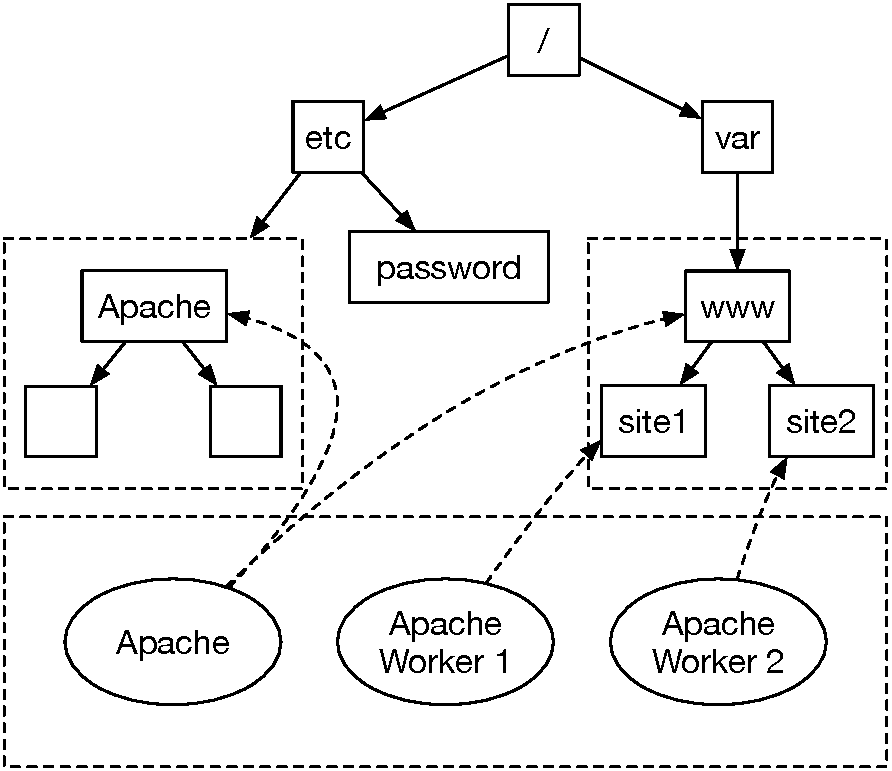
\includegraphics[width=0.65\linewidth]{imgs/fs-namespace-subsets}
  \caption{全局文件系名字空间可以被委托给沙盒进程}
  \label{fig:fd-namespace-subsets}
\end{figure}

进一步地,Capsicum拿出了自己实现capability的解决方案:尽可能复用现有的UNIX POSIX的API接口逻辑,选择拓展传统的fd(file descriptor)抽象,在其基础上进行再封装,即得到capability。这个设计比较讨巧的一点是,fd本身就具有了不可伪造的特性,且会被子进程或者通过IPC channel继承(比如fork、exec、UNIX domain socket)。而想Mac OSX和Mach对capability的管理则采取了与传统fd并列维护的策略,容易使得开发者在两者之间产生混淆与困扰。Capsicum提供新的接口cap\_new,接受fd以及一个标注权限的mask(大概有60多种)作为参数,生成对应的capability。特别地,如果参数fd本身就是capability,则新的mask必须是其子集。系统通过接口fget进行capability的权限检查,其会在内核中被转化为对应的reference,从而确保任何对该对象的访问不会绕过前述的权限检查。这里,capability可以作为目录的fd,过程中一些传递的情况被限制,使得目录的capability能够委托文件系统的名字空间的子集,如图 \ref{fig:fd-namespace-subsets}所示,以保证避免诸如chroot vulnerability的类似情况等。此外,Capsicum中禁止通过fexecve进行提权。

从实现上,Capsicum在内核服务的实现部分就进行了修改,而不是简单的对系统调用进行过滤,这样的话一个单一的限制就可以再单个地方得以完成(比如,namei);并没有独自设置一套IDL(Interface Description Language),从而可以尽可能地兼容以后程序。同时,Capsicum提供了一个运行时的底层组件,即libcapsicum。

\subsection{应用调整}
\label{sss:adoption}

由于Capsicum从设计到实现,都尽可能地保留了原有的结构,所以在应用调整这块相对来说是非常轻松的。

开发者首先需要分析程序来确定资源的依赖关系,并使其模块间以分布式系统的方式沟通,即模块间通过message-passing或者共享内存来通信,而不是地址空间。其次,一共有两种方案可供选择,一个是直接使用capability mode,另一个则是通过调用libcapsicum完成:
\begin{itemize}
	\item
	对于结构简单的程序(比如只有一个I/O循环),可以直接使用cap\_enter,这样的overhead是非常小的,样例程序可以是tcpdump
	\item
	对于已经有权限分离机制的程序,尽管其结构可能相对复杂,但是已经有了通过fd来传递的概念,通过简单的修改,同样使用cap\_enter,在安全性上可以获得显著的提升,带来的overhead也是很小的,样例程序可以是dhclient和Chromium
	\item
	而对于其他程序,在确定好边界的前提下,通过libcapsicum API来对原程序进行改写,以在保证performance的同时提升安全性,样例程序可以是gzip。
\end{itemize}

而实际上,即使不在系统级别上实现capability-based security,依旧可以从编程的角度,进行capability-oriented programming\footnote{http://wiki.c2.com/?CapabilityOrientedProgramming},其中主要需要注意的点在于(由于不是本文重点,只做简单概述):
\begin{itemize}
	\item
	不要有全局静态的可枚举状态
	\item
	对象的实例化需要划分层次,以保证在每个层次都符合POLP
	\item
	封装(即模块化)必须严格遵守
	\item
	对可信区间(trust realms)的边界有很多特殊的技巧,以防止不必要的泄露
	\item
	每一个会被暴露给client的接口都必须检查所有先决条件(precondition)
\end{itemize}

\chapter{Sandboxing 各种实现的分析与对比}
\label{s:evaluation}

\section{实现比较}
\label{ss: comparision}

\begin{figure}[!htp]
  \centering
  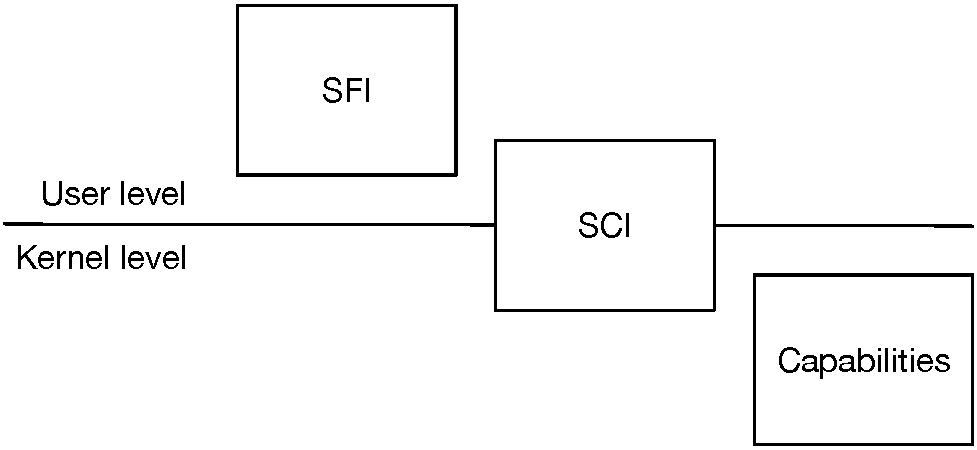
\includegraphics[width=0.7\linewidth]{imgs/difference}
  \caption{三种实现的比较}
  \label{fig:difference}
\end{figure}

在分类中,SFI 属于第一类沙箱,而 SCI 和 Capability 属于第二类沙箱。它们各自的实现如图 \ref{fig:difference} 所示,分别是实现在用户态,内核态以及在内核态和用户态都有一部分实现。其中 SFI 是完全用户态的实现,依靠二进制改写或修改编译器等等方式来进行错误的隔离。这样的实现相比于其他两种技术的实现方式,会更加简单。但是 SFI 的实现往往会依赖操作系统的 API 或者 ABI,这使得对于不同的处理器架构而言,要进行不同的实现,普适性不是很好。Native Client 最初是在 X86 架构上实现的。其后的论文 \parencite{sehr2010adapting} 介绍了 SFI 在 ARM 和 X86-64 架构上的实现方式。相比于 X86 的实现,就会有一些不同的实现思路。

而 SCI 要求在内核态和用户态都要进行一定的实现,因为 SCI 的 policy engine 往往是在用户态运行,而真正处理系统调用的逻辑是在内核中完成的。SCI 能够过滤所有不合法的系统调用,这是其主要关注的问题,也是其他两种方式实现不了的。但是 SCI 的缺点也是非常明显的:time-of-check/time-of-use 竞争问题 \parencite{bishop1996checking}。因为 SCI 在用户态检查合法性,而在内核态执行真正的系统调用,所以权限检查与系统调用的执行不是原子性的。这就带来了数据竞争的问题。在早期的 Janus 实现中,会出现全局、进程间和线程间三种数据竞争。而 Ostia 通过改变了实现的架构,解决了后两者的数据竞争的问题,对于前者,Ostia 采取了一种相对而言不太严谨的做法来规避了问题的发生,因为 Ostia 的 委托架构,使得 Agent 可以重新组织系统调用使得应用发起的系统调用遵循操作系统的惯例。但是我们认为这样有可能会导致一些对顺序敏感的应用程序在调用时产生顺序上的错误,并没有完全解决问题。

Capability其实严格来说是一种安全哲学,作为这三者中唯一可以完全植根于内核态的安全框架,其向用户暴露的主要是系统调用以及运行组件,最大的优势在于遵从POLP,做到了细粒度的AC,并维护了细粒度任务到细粒度权限的映射,从而避免了由于混淆所导致的confused deputies problem;同时,相较于传统的基于ACL的权限策略,更具灵活性。但是传统思路下实现的Capability存在明显的技术限制,且有较大的编程难度,所以很少在商用OS中得到推广。Capsicum作为被纳入FreeBSD9的一种基于Capability的安全框架,以其讨巧的设计在安全性与额外开销之间找到了一个可行的平衡点,但如何以更小的代价得到更高的安全性仍是需要不断探索的方向。

\section{性能分析}
\label{ss: analysis}

沙箱技术在提高了隔离性的同时,不可避免地为系统引入了新的 overhead。由于三者的实现不同,因此有着不同的 overhead。这三种沙箱技术的 overhead 大多体现在网络,计算和系统调用上。三者的研究论文并不是完全按照这三个不同子系统的 overhead 来进行验证与测试的,但是其测试结果从侧面反映出了在三者之上的性能损耗。

以 Janus、Ostia 为代表的 SCI 技术,关注过滤系统调用请求。因此该实现在网络和计算上的性能损耗非常小,基本可以忽略不计。Ostia 是在我们所见的论文中,唯一一个以这三方面作为不同的研究对象进行性能损耗的讨论的,Ostia 在对网络和计算的测量中,两者的 overhead 均没有超过 1\%,而在系统调用方面,改进后的 Janus \parencite{wagner1999janus} 有 8\% 的 overhead,而 Osita 因为委托架构的实现,在解决了部分数据竞争问题的同时,带来了 25\% 的 overhead。

SFI 相比于 SCI,性能损耗更多体现在计算上,而在网络和系统调用上都可以忽略不计。在计算方面,SFI 的 overhead 体现在:

\begin{itemize}
\item
使用 SFI 技术对 store 和 jmp 等指令进行保护检查。这是 SFI 性能损耗最大的一点,平均有 22\%。Native Client 对原本的实现有所改进,但是并没有质的改变,仍然是同一数量级。
\item
以及为了实现 SFI 向原本的二进制中插入的指令的长度。SFI 需要多余的指令完成检查的逻辑,因此支持 SFI 的二进制文件会比不支持 SFI 的文件多 10\% 左右的指令。
\item
相比于传统的执行多使用的寄存器数目。因为 SFI 使用了栈寄存器等,因此在寄存器数目上也存在 overhead,但这基本可以忽略不计。
\end{itemize}

综合来看,SFI 在计算上有平均 5\% 的 overhead。

以Capsicum为代表的基于capability的安全框架主要是在内核中实现,故其overhead主要可以通过三个维度来衡量:系统调用、沙盒创建,以及实际程序的执行。将相关测试结果用基于置信度为 95\%的T检验进行分析,可得:Capsicum所提供的API,相较于原生的UNIX POSIX的API,造成了大约 10\% 的overhead;而沙盒创建(即cap\_enter),达到了与chroot相似的overhead,而相较于fork,则造成了 9\% 的overhead;在实际程序的执行上,以gzip为例可见,capability所造成的overhead主要来自于诸如沙盒创建等初始阶段,所以当任务较为琐碎的时候(在gzip样例中表现为文件大小较小),capability会产生明显且非常稳定的overhead,而当任务变大时,capability版本的程序与原程序几乎没有表现出明显的性能差异。

综合来看,capability不可避免地会产生一定的overhead,且这些overhead主要来自于沙盒创建,及相关接口调用(如由fd生成相应的Capability)等,平均上有9\%左右的overhead,且能随着单个程序本身的业务逻辑的增大而得到均摊。

值得一提的是,Capsicum的作者尝试从另一个角度来看待这个问题 \parencite{capsicum}:任何安全隔离都不可避免地带来开销,换言之,任何security-critical的程序的设计者其实都默认接受了一定的overhead,所以不如以“如何用一定的overhead来换取更好的安全性”作为问题的核心。虽然这一点就测试而言,似乎该怎么测试还得怎么测试,但是我们认为,在系统设计之初就抱有这样的想法的话,不失为另辟蹊径的一种策略,可作参考。

%# -*- coding: utf-8-unix -*-
%%==================================================
%% conclusion.tex for SJTUThesis
%% Encoding: UTF-8
%%==================================================

\chapter{讨论与总结}
\label{s:tucao}

在上文中,主要探讨了三种沙箱的实现思路以及对比。本节将对沙箱技术的发展,应用以及未来的研究点进行预测和概括。

SCI 已经形成了较为成熟的方法论,自 Janus 开始,几乎所有的研究都是混合了用户态和内核态的实现。这样的实现是出于解耦保护和管理的目的,但是会导致数据竞争的问题,是数据竞争的潜在可能性与可配置性的权衡。完全从内核中实现 SCI,也是有一定的应用场景的。这样的实现会降低可配置性,但是会提高性能,同时可以彻底解决数据竞争的问题。在 Unikernel 等等场景下,操作系统中只跑一个已知的特定的应用时,可以将 SCI 实现在内核层。

SFI 在谷歌浏览器中得到了广泛的使用,Native Client 现在仍然是 Chrome 浏览器支持的特性之一。但是,它的实现思路并没有得到大家的广泛认可。Firefox 浏览器跟 Chrome 浏览器的选择不同,Native Client 重新定义了一个二进制的格式,来保证错误的隔离。而 Firefox 通过将原生的代码编译成中间代码,然后将中间代码翻译成 Javascript 语言的一个被称作 asm.js 的子集,进而实现了原生代码在浏览器中的运行。相比于 Native Client 的实现,asm.js 完整地复用了浏览器的沙箱,因此不会涉及 SFI 的相关运用。

\begin{figure}[!htp]
  \centering
  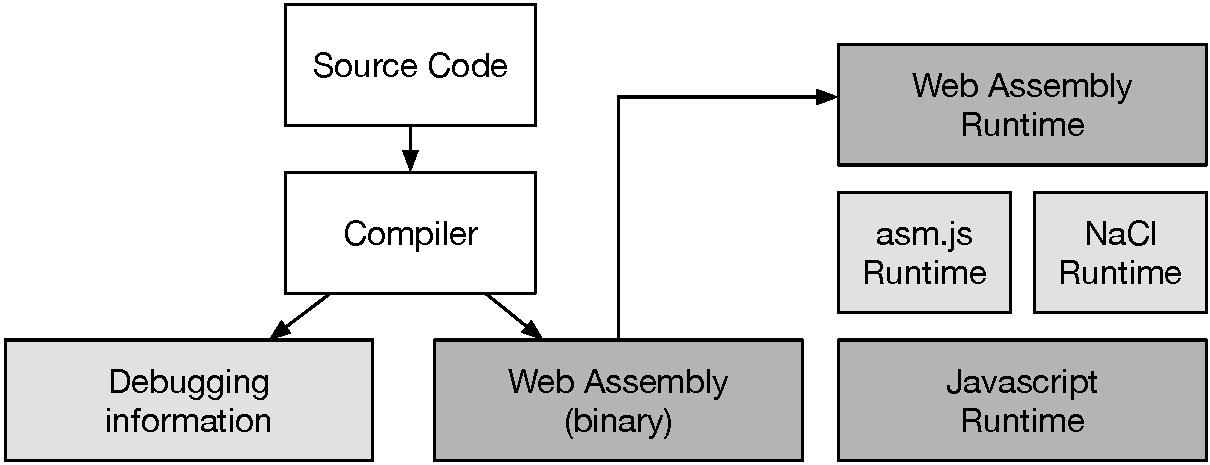
\includegraphics[width=0.7\linewidth]{imgs/wasm}
  \caption{WebAssembly 原型图}
  \label{fig:wasm}
\end{figure}

目前业界对于在浏览器中运行原生代码的解决方案,是综合了 Firefox 和 Chrome 浏览器两种思路而产生的。其主要借鉴了 asm.js 的思想,因此被称为 WebAssembly。如图 \ref{fig:wasm} 所示,WebAssembly 通过将原生代码编译为一种特殊的中间格式,然后在浏览器中执行编译产生的中间代码。WebAssembly 希望能够将运行时建立在 asm.js 和 Native Client 的抽象之上。目前 WebAssembly 已经支持将中间代码转换为 asm.js 来运行。这一方案是由 Firefox 的 asm.js 团队和 Chrome 的 Native Client 团队一起开发的,Native Client 团队因为其安全方面的特长,因此主要负责 WebAssembly 的安全与隔离。

WebAssembly 是以后 Web 发展的新趋势,也得到了谷歌、微软、苹果等公司的大力支持,以及 Javascript 之父 Brendan Eich 的背书。而 WebAssembly 目前还处于初级阶段,这其中自然存在一些安全问题。包括从编译器的代码生成环节,如何保证生成的代码是与原本的代码逻辑等价的;到在浏览器中运行时,如何安全地实现如同 Native Client 中原生代码与 Javascript 代码之间的交互,等等。这将是今后安全领域有一个新的研究点。这其中的问题未必能单独依靠沙箱技术来独立解决,由 Native Client 可知,现在的安全研究越来越多地涉及到多种技术的综合,WebAssembly 与编译器安全、操作系统安全、沙箱等等技术都有相关性。

% 研究点:移动端沙箱(Deprecated)

Capability作为另一种安全哲学,支持了细粒度的AC,其实可以被应用在很多地方。其在内核层面的实现,由于技术限制以及编程难度,并没有被商业OS们所真正采纳。而Capsicum作为其主要的内核实现,被纳入在FreeBSD 9中,并成为了Chromium在FreeBSD上的主要安全基础。可见,如何更好地权衡开销与性能,它在系统层面还有很长的路要走。退而求其次,capability-oriented programming则应运而生,即在程序设计层面应用Capability的安全哲学,其在程序设计上提出了相应的规范和要求,并得到了一定程度的认可和应用:OpenSSH, Apple's Security Server都遵循了这样的设计思路。也正因为如此,我们认为capability是三种沙箱技术中最具有实际的借鉴意义的。

这三种沙箱技术,都是属于系统领域的研究,在系统设计时,其在实现上的考量,借鉴了很多经典的计算机系统原理。Janus 在实现时,总结了宏内核、微内核以及混合内核的想法,提出了在用户态和内核态同时来实现 SCI 的想法。为了实现全方位的沙箱限制,Native Client 从各种角度,使用了各种技术来对沙箱内的代码进行限制,保证了代码的最小权限运行。Capsicum 源自最小特权原则,而且在考虑到 least astonishment 之后,选择尽可能地复用 Unix API,并且与文件描述符的抽象进行了整合,被并入了FreeBSD 9的内核中,遵循 Unyielding foundations 的规则。由此可见,一个好的系统研究并不是完全从零开始,而是面对新的问题,尽可能地使用经典的,经过时间考验的设计原理来解决,这样可以最大化系统的可用性。


\backmatter	% 文后无编号部分 

%% 参考资料
\printbibliography[heading=bibintoc]

%% 致谢、发表论文、申请专利、参与项目、简历
%% 用于盲审的论文需隐去致谢、发表论文、申请专利、参与的项目
\makeatletter

% \include{tex/patents}	  %% 申请专利
% \include{tex/resume}	  %% 个人简历

\makeatother

\end{document}
